\section{Introducción}

Es una buena costumbre comenzar cada capítulo con una sección de
introducción donde se describa lo que se va a mostrar en este
capítulo. Es más fácil escribir esta sección después de haber escrito
el capítulo completo. En este capítulo se introducen las ideas
generales para escribir un trabajo de tesis y su organización,
pensando en un trabajo de la Licenciatura en Ciencias de la
Computación de la Universidad de Sonora.

 \section{¿Como se organiza una tesis?}

 \subsection{Numero de capítulos}

 ¿Cuantos capítulos son necesarios para una tesis? Esto varía mucho
 dependiendo de la forma en que está organizado el trabajo, en común
 acuerdo con el director de tesis. Normalmente es mejor poner uno o
 dos capítulos que describan el estado del arte, las técnicas o las
 bases teóricas del trabajo a realizar, y que se utilizarán en el
 resto de la tesis.  En estos capítulos no se presentan ideas nuevas
 ni el desarrollo que más costó trabajo, solo las bases necesarias
 para entender el trabajo realizado. Se puede considerar una especie
 de revisión bibliográfica y suelen tener la mayor parte de las
 referencias bibliográficas de todo el trabajo escrito.

 En los capítulos subsecuentes, lo normal es ser muy específico y
 desarrollar con detalle el trabajo realizado, tanto si es un
 desarrollo teórico, un desarrollo tecnológico, como si es simulación
 o experimentación real. Estos capítulos suelen ser relativamente
 cortos y con muchas imágenes, gráficas y tablas en el caso de
 trabajos aplicados.

 Es común que una tesis de licenciatura tenga 3 capítulos, sin contar
 el capítulo de introducción y las conclusiones generales. Es importante resaltar que esto
 depende mucho de la naturaleza del trabajo desarrollado y debe ser
 establecido de antemano en común acuerdo entre el director de tesis y
 el estudiante. Igualmente, cabe resaltar que es normal, durante el
 desarrollo de la tesis (y más específicamente durante su redacción)
 que se considere agregar y/o quitar capítulos sobre el proyecto
 original.

 \subsection{¿Y la cantidad de páginas de una tesis?}

 ¿Cuantas cuartillas debe tener una tesis? Es una pregunta muy normal
 que se hacen todo mundo cuando comienza la fase de redacción. Las
 páginas correctas son \emph{las que sean necesarias para explicar el
   trabajo desarrollado}. Este número cambia mucho dependiendo de la
 disciplina. Por ejemplo, los trabajos en computación teóricas suelen
 ser muy cortos (unas 30 páginas para una tesis de licenciatura),
 mientras los trabajos enfocados a ingeniería de \emph{software}
 tienden a ser muy extensos (de 80 a 100 páginas).

 Es recomendable hacer un trabajo breve, normalmente entre 30 y 50
 páginas. Sin embargo, no existe una limitante, si el trabajo, por su
 naturaleza, requiere que sea explicado en más espacio, o naturalmente
 se tiende a escribir mucho. Se puede extender el trabajo de tesis
 \emph{hasta 100 páginas como máximo}. Es importante tomar en cuenta que en
 muchas Universidades del mundo, se tiende a limitar los trabajos de
 tesis de doctorado a 150 páginas como máximo con todo y apéndices. Un
 trabajo muy largo no significa que sea mejor.


 \subsection{¿Y como organizar el trabajo?}

 Para organizar el trabajo, \LaTeX contempla el uso de
 \verb+\section+, \verb+\subsection+, \verb+\subsubsection+ y
 \verb+\paragraph+. Si bien en este capítulo se hace uso de la mayoría
 de estos bloques con fines ilustrativos, en general es mejor tratar
 de mantener la organización del trabajo hasta
 \verb+\subsection+. Considere el uso de listas, enumeraciones y
 descripciones si requiere escribir muchos párrafos cortos con títulos
 en \verb+\subsubsection+ o \verb+\paragraph+. Igualmente, evite el
 uso excesivo de listas en un trabajo, ya que esto solo denota una
 pobre capacidad para expresar ideas en párrafos de texto.


 \section{Escribir un trabajo en \LaTeX}


Para realizar un trabajo científico en el área de Ciencias de la
Computación, especialmente en las ramas de computación teórica,
computo científico e inteligencia artificial, es normal utilizar
\LaTeX. Se asume que es normal que un estudiante que está preparando
una tesis de licenciatura en Ciencias de la Computación tenga
experiencia previa en escribir trabajos más pequeños en \LaTeX. 

Un buen comienzo para escribir un trabajo en \LaTeX, es buscar en otros trabajos un
ejemplo de algo similar a lo que queremos hacer, y luego adaptarlo a
las necesidades particulares. Por esta razón, en esta sección se
incluyen ejemplos para la inserción de figuras, cuadros, listas y
descripciones. Utilice estas plantillas, pero tenga cuidado en su
uso. Un problema muy común es el copiar la plantilla para la inserción
de figuras o cuadros, sin cambiar el comando \verb+\label+, por lo que
a la hora de compilar, se hace referencia en todo el documento a una
sola imagen.


\subsection{Inserción de figuras}


Las imágenes soportadas en la clase (y compiladas con \verb+pdflatex+)
son PNG, JPG, GIF y PDF de preferencia. Evitar utilizar imágenes de
tipo EPS. La figura \ref{fig:pdf} es un ejemplo de inserción de un
gráfico en PDF. La figura \ref{fig:png} y la figura \ref{fig:jpg} son
ejemplo para insertar imagenes en PNG y JPG respectivamente. La
leyenda de las figuras \emph{siempre} se encuentra por abajo de la
figura o imagen. 

\begin{figure}[tb!]
	\centering
    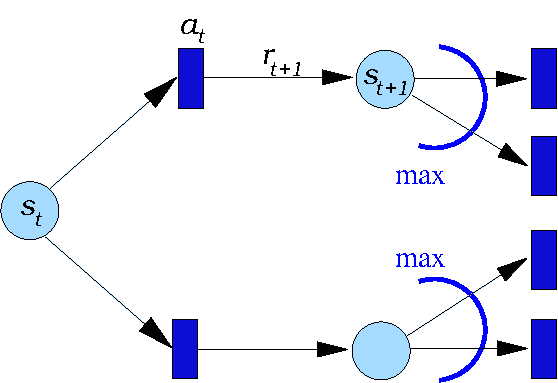
\includegraphics[width=0.5\textwidth]{tesislcc/ejemplo1.pdf}
    \caption{Ejemplo de inserción de una imagen en PDF}
    \label{fig:pdf}
\end{figure}

\begin{figure}[htb!]
	\centering
    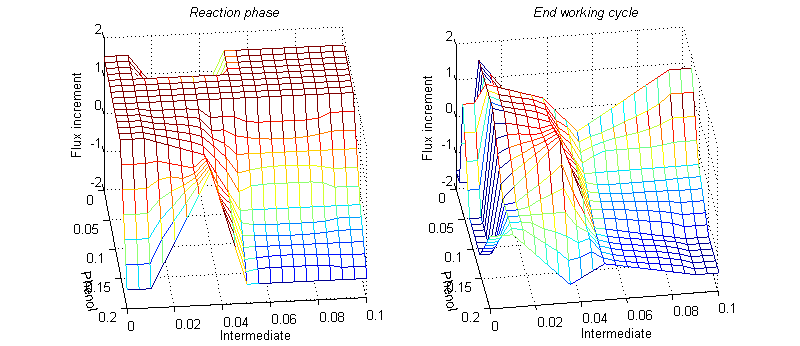
\includegraphics[width=0.7\textwidth]{tesislcc/ejemplo2.png}
    \caption{La leyenda de la figura siempre va abajo de ésta}
    \label{fig:png}
\end{figure}

\begin{figure}[htb!]
	\centering
    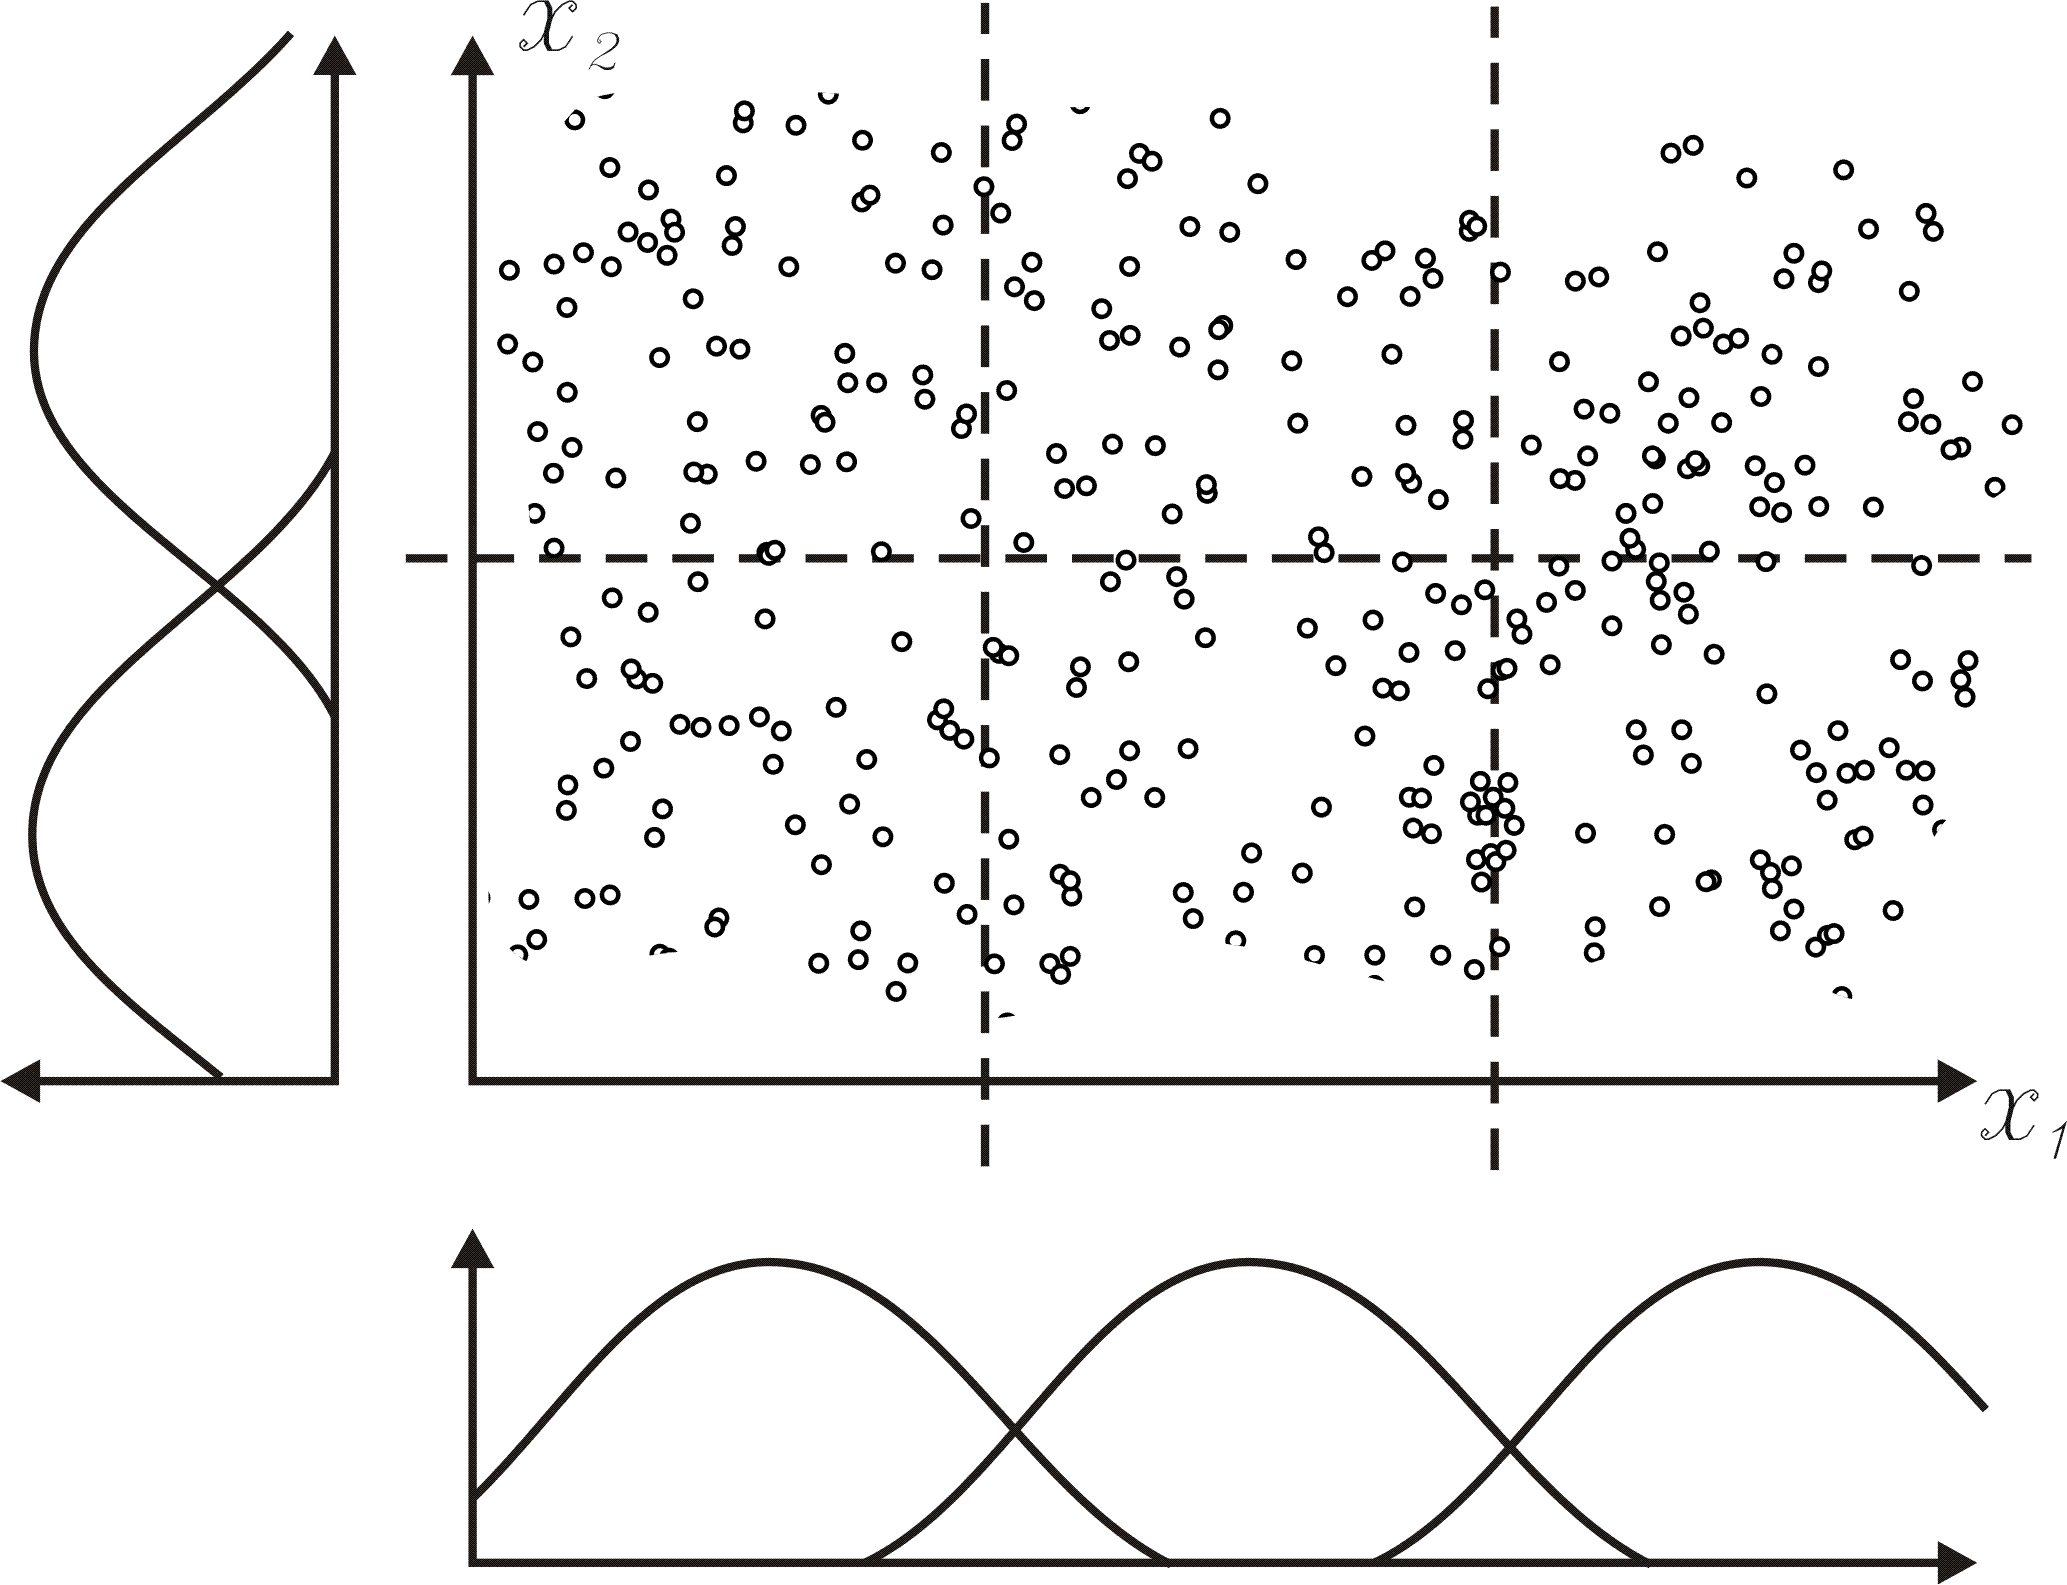
\includegraphics[width=0.5\textwidth]{tesislcc/ejemplo3.jpg}
    \caption{Procure que la leyenda explique claramente el
        título de la figura, aunque sea necesario que sea una leyenda
        larga que ocupe varias líneas}
    \label{fig:jpg}
\end{figure}


La colocación de una figura se puede controlar con los commandos
\texttt{h,t,b,p} (de \emph{here},\emph{top},\emph{bottom},\emph{page})
utilizando el orden como prioridad. Si por alguna extraña razón se
desea colocar una figura en un lugar específico del texto, se coloca
con el comando \texttt{H} (\emph{here} pero mandatorio). En general (y
esto es tanto para las tablas como para las figuras) no debe mucho
preocupar si las figuras se colocan en páginas diferentes que en las
que se hace referencia de ellas. 

Editorialmente esto es válido y recomendable. \LaTeX \ lo
que intenta es colocar las figuras siempre arriba de una página y evitar que el
porcentaje de texto en una página sea menor al 30\% de su contenido.
En la clase de tesis\verb+tesislcc+ se amplió el margen para
poder colocar figuras mas grandes, o varias figuras en una página. 

Es muy importante que se haga
referencia de todas las figuras en el texto y se discuta sobre ellas,
así sea sólo una línea de texto. Si no es posible hacer referencia de
una figura en el texto, significa que no es necesario que se encuentre
en el documento.

Otra práctica común y que suele ayudar mucho, sobre todo cuando la
tesis se encuentra bastante avanzada o cuando se piden cambios por
parte de los revisores, es el utilizar uno o varios directorios en los cuales se guarden las
figuras. Esto es especialmente importante en trabajos experimentales o
de desarrollo tecnológico que típicamente llevan varias capturas de
pantallas o muchas gráficas. En este ejemplo, las figuras se
encuentran agrupadas en un subdirectorio \texttt{figuras} (haciendo
gala de falta de imaginación).



\subsection{Inserción de cuadros}



Por abuso del idioma, tendemos a decirle en español tablas a lo que de
manera correcta deberíamos nombrar como \emph{cuadros}. Esto se debe a
que en inglés se les conoce como \emph{tables}. La leyenda de los
cuadros \emph{siempre} se encuentra arriba del cuadro (al revés que en las
figuras). El cuadro \ref{Ta:primer ejemplo} es un ejemplo típico de
cuadro. Es importante siempre citar y explicar un cuadro en el texto,
de otra manera significa que no es una información  necesaria. 


\begin{table}
  \centering
  \caption{Tabla de muestra para la tesis}
  \label{Ta:primer ejemplo}
  \vspace{.1cm}
  
  \begin{tabular}{|l|c|r|}
    \hline
    % after \\: \hline or \cline{col1-col2} \cline{col3-col4} ...
    Texto & Formulas & Numero \\
    \hline\hline
    Cosa & $\sqrt{x^2 + b^2}$ & 3.1416 \\
    Pasto & $3.2 + e^{-t}$ & 4578 \\
    \hline
  \end{tabular}
\end{table}

Todas las referencias (a figuras, cuadros, secciones, etc.) se deben
hacer utilizando los comandos \verb+label+ (para marcar un entorno) y
\verb+ref+ (para citarlo en el texto). En documentos muy grandes esto
es muy importante, ya que si se elimina o se agrega un cuadro o
figura, no es necesario reescribir todo el texto y revisar que se
haga referencia correcta de ellos en el texto.



\subsection{Escribiendo matemáticas}


Todos los estudiantes que realizan una tesis y requieren
de formalismo matemático, en general escogen \LaTeX como entorno de edición
preferencialmente, ya que la calidad tipográfica, como la facilidad
para incluir notación matematica en el texto, hacen que, en términos
generales, sea mucho más fácil escribir una tesis en \LaTeX que en un
entorno tipo WYSIWYG como \emph{World}. En esta sección se asume que
el lector se encuentra familiarizado con el uso de \LaTeX y el uso de
notación matemática, por lo que solamente se realizarán pequeñas recomendaciones. 





\section{Conclusiones}
En general, no es nada mala idea poner una última sección con
conclusiones de lo que se mostró en el capítulo. Para los revisores
y/o lectores del trabajo, les facilita mucho realizar una primer
hojeada al documento.

%%% Local Variables: 
%%% mode: latex
%%% TeX-master: "Tesis"
%%% End: 
